\documentclass[a4paper, 12pt]{article}
%\usepackage[utf8]{inputenc} 
\usepackage[frenchb]{babel}
\usepackage{fullpage}
\usepackage[T1]{fontenc} 
\usepackage{graphicx}  
\usepackage[final]{pdfpages}
\usepackage{amsmath, amssymb, wasysym, amsthm}
\usepackage{listingsutf8}
\usepackage{lmodern}
\usepackage{tikz}
\usepackage{pgfplots}

\newtheorem{mydef}{Définition}
\newtheorem{thm}{Théorème}
\newtheorem{lem}{Lemme}
\newtheorem{cor}{Corollaire}
\newtheorem{prop}{Propriété}

\title{Rapport de Méthodes approchées.}
\author{Dyce William, Loukil Amal, Ouazzani-chahdi Sabrina : \\ M1 MOCA}
\date{semestre 2 : 2011-2012}

\begin{document} 

\maketitle

\begin{abstract}
  Le présent document consiste en un mémoire au sujet
  d'exercices à la fois théoriques et pratiques sur diverses
  problèmatiques liées à l'étude de méthodes approchées pour la
  résolution de problèmes NP-difficiles. 
\end{abstract}
\vspace{2cm}
\textit{Travelling salesman's problem :}
\begin{figure}[h!]
\centering
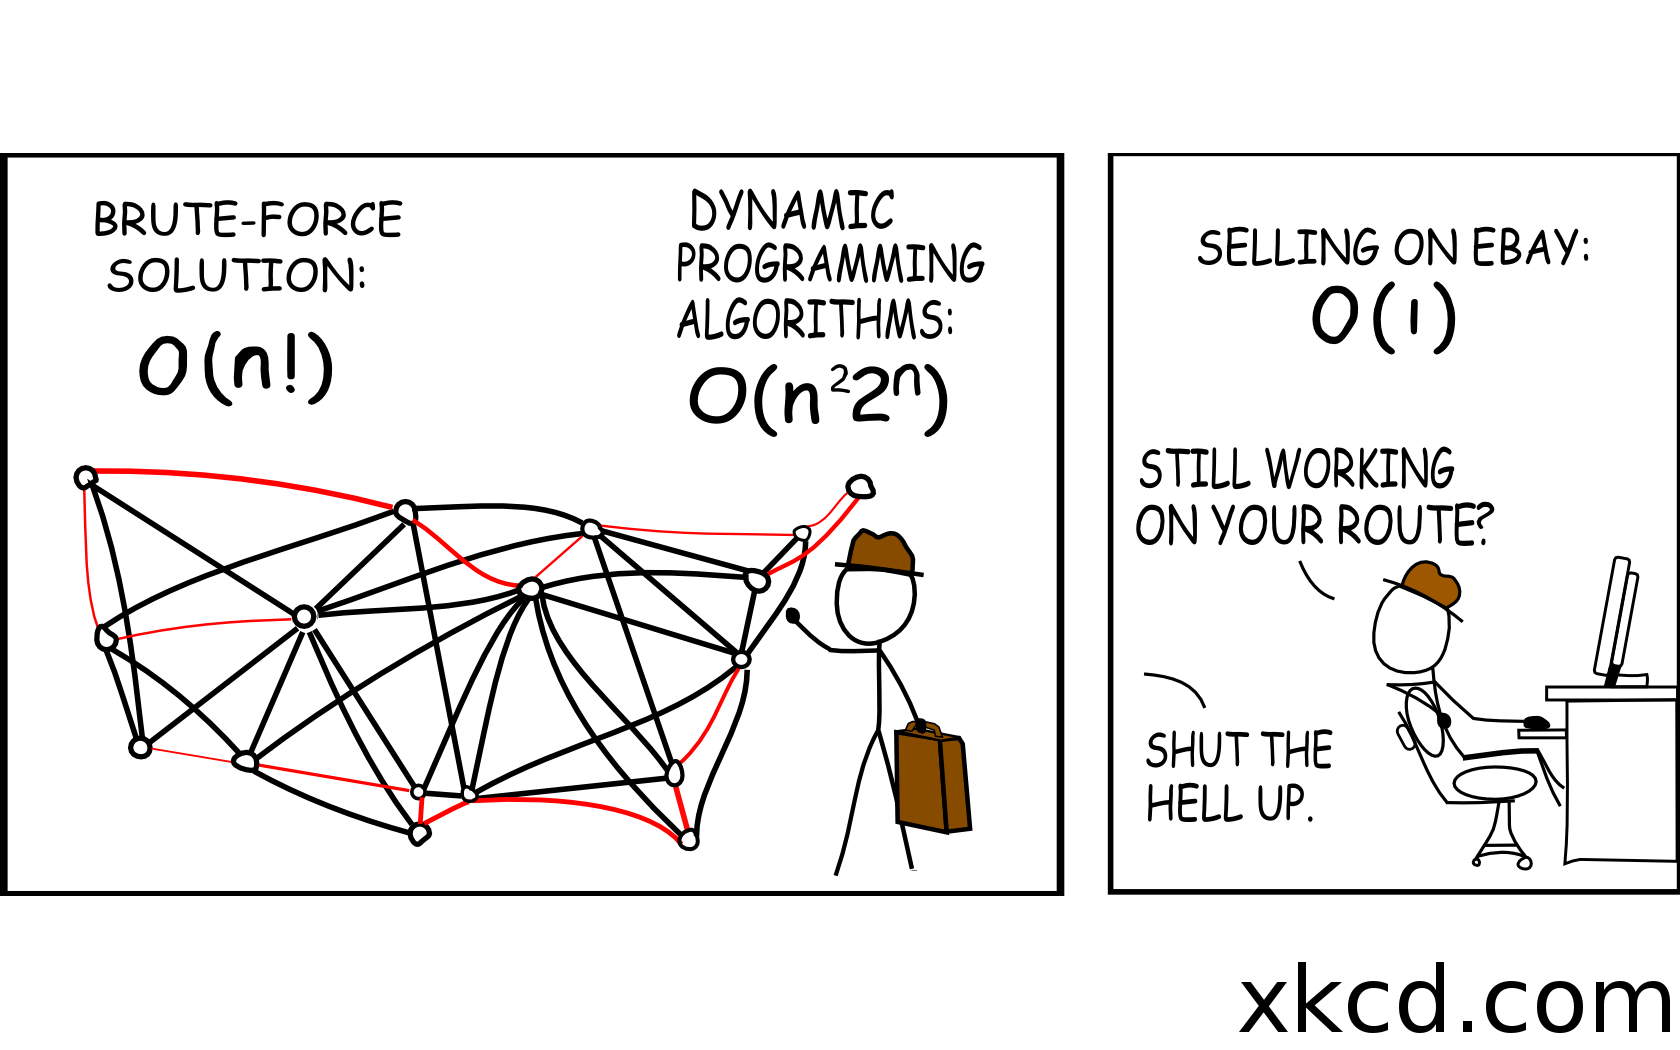
\includegraphics[height = 9cm]{commerce.png}
\end{figure}


\pagebreak

\tableofcontents

\pagebreak

\listoffigures

\listoftables
\pagebreak

\section{Généralités et notations}

\section{Partie théorique}

\subsection{Programmation linéaire en nombres entiers}

\subsubsection*{Exercice 1}

\paragraph{Question 1}

\begin{itemize}
\item[] a) Le programme linéaire en nombre entier présenté dans
  l'énoncé se justifie de la manière suivante~:
\begin{itemize}
\item $x_j \in \{0,1\}, j=1..n$ car on a le choix binaire entre prendre un
  sommet (donc le compter avec 1), ou ne pas le prendre (ne pas le
  compter avec 0, élement neutre de l'addition). Il y a bien
  évidemment n sommets, d'où l'indexation de 1 à n.
\item $min z = \sum^n _{i=1} x_i$ car on souhaite minimiser le nombre
  de sommets pris.
\item $x_r + x_s \geq 1$ car au moins un sommet doit être pris pour
  couvrir une arête.
\end{itemize}
Ces trois conditions décrivent donc bien le problème de la couverture minimale.
\item[] b) exemple du triangle (à faire en dessin), cette condition
  n'est donc pas suffisante.
\item[] c) Montrons par l'absurde que le programme linéaire en nombres
  entiers est une borne inférieure de toute solution optimale.
\begin{proof}
Supposons que pour une instance donnée, on ait une solution
  optimale de vertex cover qui soit meilleure que PLNE. Cela veut donc
  dire que PLNE garde au au moins un sommet <<~en trop~>>. Or PLNE
  devrait minimiser le nombre de sommets. Le résultat est donc absurde
  et contredit notre hypothèse de départ.
\end{proof}
\item[] d) Nous allons ici montrer de deux manières différentes que la
  relaxation des contraintes d'intégrité implique $x_r \geq
  \frac{1}{2}$ ou $x_s \geq \frac{1}{2}$.
\begin{itemize}
\item Première démonstration.
\begin{proof}
On veut, malgré la relaxation des contraintes d'intégrité, conserver
l'inégalité $x_r + x_s \geq 1$. Ainsi, on a $\neg (x_r + x_s < 1)$
d'où $\neg (x_r < \frac{1}{2} \wedge x_s < \frac{1}{2})$, et donc
($x_r \geq \frac{1}{2} \vee x_s \geq \frac{1}{2}) $ de par la loi de
De Morgan.
\end{proof}
\item Deuxième démonstration.
\begin{proof}
On sait que $A \Rightarrow B \equiv \neg A \vee B$. 
Or, pour respecter l'inégalité $x_r + x_s \geq 1$, on a $(x_r <
\frac{1}{2} \Rightarrow x_s \geq \frac{1}{2})$. On a ainsi $(x_r \geq
\frac{1}{2} \vee x_s \geq \frac{1}{2})$. 
\end{proof}
\end{itemize}
\item[] e) Montrons que l'algorithme 1 conduit à un algorithme
  approché avec une performance relative de de deux. 
\begin{proof}
Soit $C^{*}$ une solution optimale du problème de la couverture de
sommet. Soit $C$ la solution donnée par l'algorithme. 
TODO
\end{proof}
\item[] f)
\begin{itemize}
\item i)
Le programme linéaire correspondant à rajouter un poids aux arêtes au
problème du vertex cover est le suivant~:
\begin{itemize}
\item  $x_j \in \{0,1\}, j=1..n$,  TODO
\item TODO écriture matricielle
\item TODO démo 2-approché
\end{itemize}
\item ii)
\item iii)
\end{itemize}
\end{itemize}

\paragraph{Question 2}

\begin{itemize}
\item[] a) Montrons que l'algorithme 2 est 2-approché.
\begin{proof}
Soit $C^{*}$ une solution optimale du problème de la couverture de
sommet. Soit $C$ la solution donnée par l'algorithme. 
\begin{itemize}
\item[] $|M| \leq C^{*}$ car deux arêtes adjacentes ne peuvent être
  couvertes par un même sommet.
\item[] $C^{*} \leq C = 2 |M|$ car une arête a deux sommets.
\item[] On a donc $\frac{C}{C^{*}} \leq \frac{2|M|}{|M|} = 2$.
\end{itemize}
\end{proof}
\item[] b) Il suffit de prendre $C_4$.
\item[] c) 
\begin{itemize}
\item[] Dans le pire des cas donné à la figure 1, l'algorithme renvoie
  une solution $C$ de taille 8. Or la solution optimale $C^*$ pour cette
  instance est de taille 5. En effet, aucun des sommets de plus haut
  degré n'est inclus dans $C^{*}$. Le choix du sommet de plus haut
  degré n'est donc pas une bonne heuristique. 
\item[] En revanche, on peut remarquer que cet algorithme trouve la
  solution optimale sur $C_4$ (qui était le cas limite de l'algorithme 2).
\end{itemize}
\end{itemize}

\subsubsection*{Exercice 2}

\paragraph{Question 1}

Nous proposons la modélisation suivante en programmation linéaire en
nombres entiers pour le problème de la couverture d'ensembles~:
\begin{equation}
\begin{cases}
min \sum_{j \in I} \omega_j \\
\sum_{i=1}^{n} \sum_{j=1}^{m} x_{ij} \geq 1  avec i=1, \dots, n \\
\omega_j \geq 0 \\
\end{cases}
\end{equation}
avec $x_{ij} = 1$ si l'objet $e_i$ est pris dans l'ensemble $S_j$, 0 sinon.
\paragraph{Question 2}

\paragraph{Question 3}

\paragraph{Question 4}

\paragraph{Question 5}

Quand $f_i = 2$, $e_i$ appartient à deux sous-ensembles. On retrouve
donc le problème de la couverture de sommets par des arêtes. En effet,
un sommet représente ici un élément, et une arête un sous-ensemble à
deux éléments.

\subsubsection*{Exercice 3}

\paragraph{Question 1}Le programme linéaire en nombres entiers qui modélise le
  problème du couplage maximum de poids minimum est le suivant~:
  (notons $u_{ij}$ les arêtes du graphe)
\begin{itemize}
\item $u_{ij} \in \{0, 1\}$ car on prend une arête ou on ne la prend pas.
\item to do
\item todo
\item todo
\end{itemize}

\paragraph{Question 2}
\paragraph{Question 3}
\paragraph{Question 4}
\paragraph{Question 5}
La formulation initialement proposée n'est pas pertinente car elle ne couvre pas tous les cas. On peut ainsi considérer
les contre-exemples suivants~: TODO !

\subsection{Problèmes appartenant à la classe APX}

\subsubsection*{Exercice 4}

\paragraph{Question 1}

\subsection{Constructions de PTAS}

\subsubsection*{Exercice 5}

\subsubsection*{Exercice 6}

\subsection{Utilisation de méthodes exactes}

\subsubsection*{Exercice 7}

\paragraph{Sur le problème de la partition}

\begin{itemize}
\item a) La condition nécessaire sur la somme des poids des $n$ objets
  est la suivante~: on veut $\sum_{a \in A'} p(a)= \sum_{a \in A
    \backslash A'}$
\item b) 
\begin{itemize}
\item i) La formule qui lie les lignes $i$, $i-1$ et $p(a_i)$ est $A_i
  := A_{i-1} + A_{i tq p(a_i)} $ TODO.
\item ii) TODO
\item iii) Nous proposons les deux algorithmes suivants. TODO
\end{itemize}
\item c) La complexité est donc $O(n\times P)$.
\item d) Nous proposons les traces suivantes pour nos algorithmes~: TODO
\end{itemize}

\paragraph{Le problème du sac à dos}
\begin{itemize}
\item a) Nous justifions les formules proposées en énonçant que l'on
  prend le maximum des $x_ju_j$ pour $j$ de 1 à $k-1$ en enlevant le
  poids de l'objet $x_k$, et l'on rajoute à $x_ju_j$ l'utilité de
  l'objet en cours.
\item b) TODO
\item c) TODO
\end{itemize}

\paragraph{Le problème du voyageur de commerce}

\subsubsection*{Exercice 8}

\subsection{Méthode Primal-Dual}

\subsubsection*{Exercice 9}

cf p86

\subsection{Borne de non-approximation}

\subsubsection*{Exercice 10}

\subsubsection*{Exercice 11}

\paragraph{Question 1~:}

Les deux problèmes considérés sont NP-complets. Plus exactement, la
coloration de sommet est un problème non-APX tandis que la coloration
d'arêtes est un problème APX. 

\paragraph{Question 2~:}
\begin{itemize}
\item Si $OPT(I) \leq 3$ alors on a
\begin{equation}
A(I) \leq \frac{4}{3}OPT(I) 
\end{equation}
TODO !!!
\item
\end{itemize}

\paragraph{Question 3~:}

\subsection{Comparaison de méthodes}

\subsubsection*{Exercice 12}

\paragraph{Question 1}

Vous trouverez sur le graphique ci-dessous une représentation du
polytope associé aux équations de $PL_0$ (aire située à la fois sous la courbe
bleue et sous la courbe rouge).

\begin{figure}[h!]
\centering
\begin{tikzpicture}[scale=1.2]
    \begin{axis}[title=PL, xlabel=x1, ylabel=x2]
      \addplot
        table[col sep=comma]{equ1.csv};
        \addplot
        table[col sep=comma]{equ2.csv};
        \addplot
        table[col sep=comma]{abs.csv};
        \addplot
        table[col sep=comma]{ord.csv};
        \legend{contrainte1, contrainte2}
    \end{axis}
\end{tikzpicture}
\caption{Polytope exercice 12}
\end{figure}

\paragraph{Question 2}
De manière graphique, on trouve environ $x_1 = 1.5$, $x_2 = 3$, $z = 6$.

\paragraph{Question 3}

Résolution du problème donné par la méthode du simplexe.

\begin{table}[h!]	
\centering
	\begin{tabular}{|c|c|c|c|c|c|}
	\hline
      & c & 2 & 1 & 0 & 0 \\ 
      \cline{2-6}
       &  & $x_{1}$ & $x_{2}$  & $x_{3}$  & $x_{4}$ \\
       \hline
   0 & $x_{3}$  $=$ 17 & 2 & 5 & 1 & 0 \\
      \hline
	0 & $x_{4}$ $=$ 10  & 3 & 2 & 0 & 1 \\
	  \hline
	 & Z($x$)$=$ 0 & -2 & -1 & 0 & 0\\
	  \hline
	\end{tabular}
\caption {Tableau 1 du simplex}	
\centering
	\begin{tabular}{|c|c|c|c|c|c|}
	\hline
      & c & 2 & 1 & 0 & 0 \\ 
      \cline{2-6}
       &  & $x_{1}$ & $x_{2}$  & $x_{3}$  & $x_{4}$ \\
       \hline
   0 & $x_{3}$  $=$ $\frac{31}{3}$ & 0 & $\frac{11}{3}$ & 1 & $\frac{-2}{3}$ \\
      \hline
	2 & $x_{1}$ $=$ $\frac{10}{3}$  & 1 & $\frac{2}{3}$ & 0 & $\frac{1}{3}$ \\
	  \hline
	 & Z($x$)$=$ $\frac{20}{3}$ & 0 & $\frac{1}{3}$ & 0 & $\frac{2}{3}$\\
	  \hline
	\end{tabular}
\caption {Tableau 2 du simplex}
\end{table}



\paragraph{Question 4, a) Branch and Bound}
\begin{itemize}
\item Nous utilisons la solution initiale suivante~:
\begin{equation}
\begin{cases}
x_1 = \frac{10}{3} \\
x_2 = 0 \\
x_3 = \frac{31}{3} \\
x_4 = 0 \\
z(x) = \frac{20}{3} \\
\end{cases}
\end{equation}
\item Nous procédons ensuite à la troncature suivante pour obtenir la
  borne inférieure de notre programme en nombres entiers.
\begin{equation}
\begin{cases}
x_1 = 3 \\
x_2 = 0 \\
z(x) = 2 \times 3 + 0 = 6 \\
\end{cases}
\end{equation}
\item Effectuons désormais un branchement sur $x_1$.
\end{itemize}
 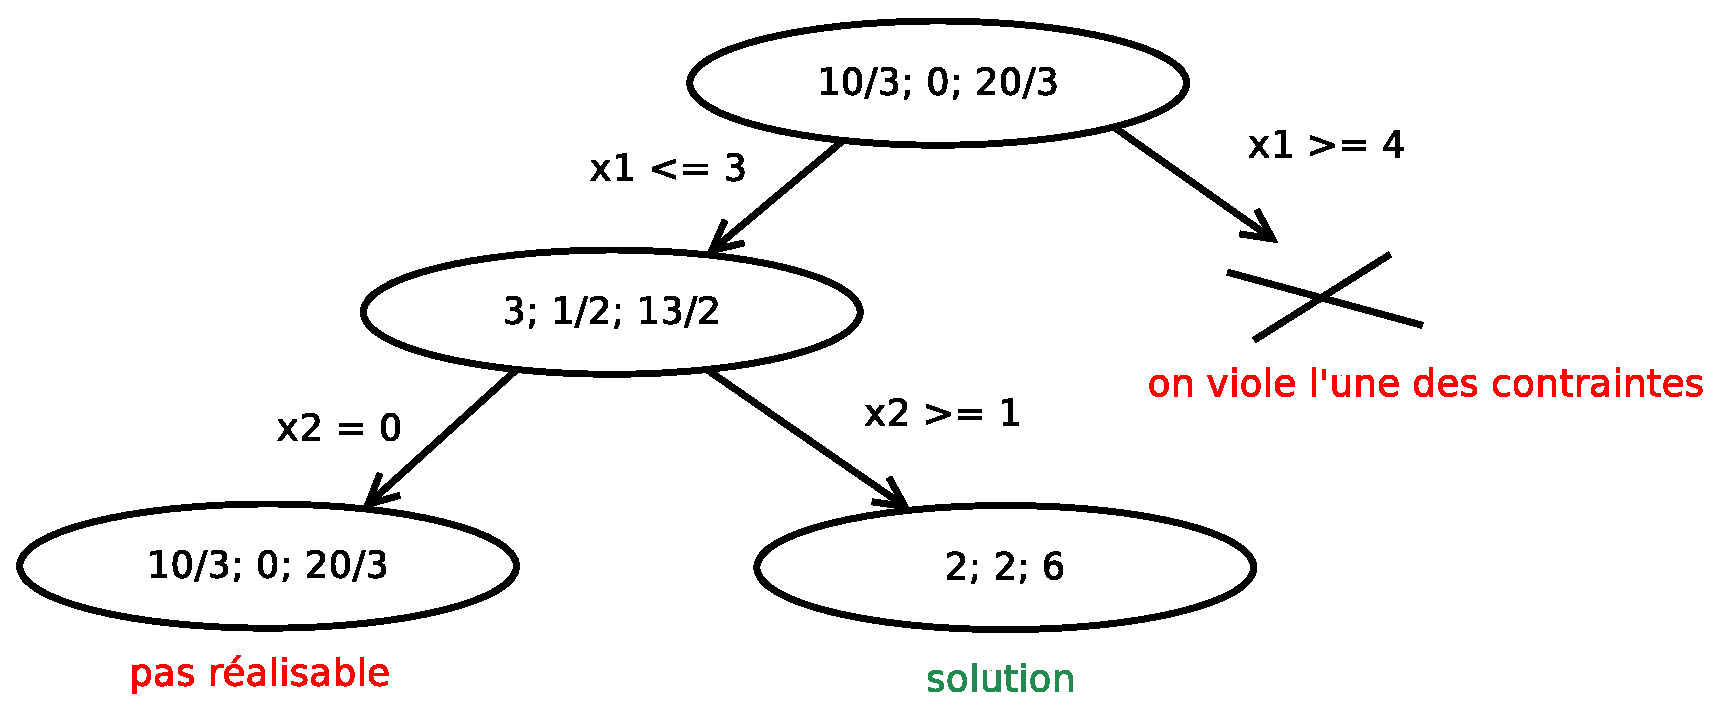
\includegraphics[height=60mm]{branchAndBound.eps}
\paragraph{Question 4, b) Branch and Cut}

Vous trouvez ci dessous les différents étapes des tableaux de la
méthode de Branch and Cut. \\
Les étapes intermédiaires sont les suivantes~:
\begin{itemize}
\item on commence par reprendre les résultats de la question
  concernant la résolution par le simplexe, puis l'on fixe la deuxième
  ligne, d'où $i = 2$.
\item $x_2$ et $x_4$ sont les variables qui ne sont pas en base. On
  peut donc écrire $\frac{2}{3} x_2 + \frac{1}{3} x_4 \geq
  \frac{1}{3}$.
\item Graphiquement, cela correspond à $x_1 \leq 3$ car on a 
\begin{equation}
\begin{cases}
2x_1 + 5x_2 + x_3  = 17 \\
3x_1 + 2x_2 + x_4  = 10 \\
\end{cases}
\\
\Rightarrow x_4  = 10 - 3x_1 - 2x_2 
\end{equation}
Ainsi, en remplaçant $x_4$ dans l'équation de l'item précédent, on a
\\
$\frac{2}{3}x_2 + \frac{1}{3}(10-3x_1-2x_2) \geq \frac{1}{3}$ \\
$\frac{2}{3}x_2 + \frac{10}{3} - x_1 - \frac{2}{3}x_2 \geq
\frac{1}{3}$ \\
$\frac{10}{3} - x_1 \geq \frac{1}{3}$ \\
$-x_1 \geq \frac{-9}{3} = -3$ \\
$\Rightarrow x_1 \leq 3$.
\item On rajoute la nouvelle contrainte obtenue dans notre tableau du
  simplexe, que nous résolvons alors par la méthode à deux phases.
\end{itemize}

TODO : étapes intermédiaires !!

\begin{table}[h!]	
\centering
	\begin{tabular}{|c|c|c|c|c|c|c|c|}
	\hline
      & c & 0 & 0 & 0 & 0 & 0 & -1 \\ 
      \cline{2-8}
       &  & $x_{1}$ & $x_{2}$  & $x_{3}$  & $x_{4}$ & $x_{5}$ & $y$ \\
       \hline
   0 & $x_{3}$  $=$ $\frac{31}{3}$ & 0 & $\frac{11}{3}$ & 1 & $\frac{-2}{3}$ & 0 & 0 \\
      \hline
	0 & $x_{1}$ $=$ $\frac{10}{3}$  & 1 & $\frac{2}{3}$ & 0 & $\frac{1}{3}$ & 0 & 0 \\
	  \hline
	  -1 & $y$ $=$ $\frac{1}{3}$  & 0 & $\frac{2}{3}$ & 0 & $\frac{1}{3}$ & -1 & 1 \\
	    \hline
	 $\frac{-1}{3}$ & Z($x$)$=$ 0 & 0 & $\frac{-2}{3}$ & 0 & $\frac{-1}{3}$ & 1 & 0\\
	  \hline
	\end{tabular}
\caption {Tableau 1 des coupes de Gomory}
\end{table}
\begin{table}[h!]	
\centering
	\begin{tabular}{|c|c|c|c|c|c|c|}
	\hline
      & c & 2 & 1 & 0 & 0 & 0 \\ 
      \cline{2-7}
       &  & $x_{1}$ & $x_{2}$  & $x_{3}$  & $x_{4}$ & $x_{5}$ \\
       \hline
   0 & $x_{3}$  $=$ $\frac{31}{3}$ & 0 & $\frac{11}{3}$ & 1 & $\frac{-2}{3}$ & 0 \\
      \hline
	2 & $x_{1}$ $=$ $\frac{10}{3}$  & 1 & $\frac{2}{3}$ & 0 & $\frac{1}{3}$ & 0 \\
	  \hline
	0 & $y$ $=$ $\frac{1}{3}$  & 0 & $\frac{2}{3}$ & 0 & $\frac{1}{3}$ & -1 \\
	  \hline
	 & Z($x$)$=$ $\frac{20}{3}$ & 0 & $\frac{-2}{3}$ & 0 & $\frac{-1}{3}$ & 1\\
	  \hline
	\end{tabular}
\caption {Tableau 1 de la méthode à deux phases}
\end{table}
\begin{table}[h!]	
\centering
	\begin{tabular}{|c|c|c|c|c|c|c|}
	\hline
      & c & 2 & 1 & 0 & 0 & 0 \\ 
      \cline{2-7}
       &  & $x_{1}$ & $x_{2}$  & $x_{3}$  & $x_{4}$ & $x_{5}$ \\
       \hline
   0 & $x_{3}$  $=$ $\frac{17}{2}$ & 0 & 0 & 1 & $\frac{-15}{6}$ & $\frac{11}{2}$ \\
      \hline
	2 & $x_{1}$ $=$ 3 & 1 & 0 & 0 & 0 & 1 \\
	  \hline
	1 & $x_{2}$ $=$ $\frac{1}{2}$  & 0 & 1 & 0 & $\frac{1}{2}$ & $\frac{-3}{2}$\\
	  \hline
	 & Z($x$)$=$ $\frac{13}{2}$ & 0 & 0 & 0 & $\frac{1}{2}$ & $\frac{1}{2}$\\
	  \hline
	\end{tabular}
\caption {Tableau 2 de la méthode à deux phases}
\end{table}

\section{Partie pratique}

\subsection{Programmation dynamique}

\subsection{Branch and bound}

\end{document}
